\documentclass[10pt,letterpaper,twoside]{article}
\usepackage{code/manuscript_assets/researchpreprint}
\usepackage[T1]{fontenc}
\usepackage{amsmath,amssymb,amsthm,bm}
\usepackage{booktabs}
\usepackage{graphicx}
\usepackage{microtype}
\usepackage{url}
\usepackage[hidelinks]{hyperref}
\setlength{\emergencystretch}{3em}

\newtheorem{theorem}{Theorem}
\newcommand{\norm}[1]{\left\lVert #1\right\rVert}
\newcommand{\LearningTasks}{48}
\newcommand{\UniqueLabels}{5}
\newcommand{\UniqueFeatures}{34}
\newcommand{\GOneVertices}{800}
\newcommand{\GOneEdges}{19,176}
\newcommand{\GEightyOneVertices}{20,000}
\newcommand{\GEightyOneEdges}{40,000}
\newcommand{\MeanConstantMSE}{0.09109}
\newcommand{\MeanRidgeMSE}{0.08150}
\newcommand{\MeanKNNMSE}{0.00137}
\newcommand{\MeanTieKNNMSE}{0.00072}
\newcommand{\MeanKRRMSE}{0.00541}
\newcommand{\MeanBlendMSE}{0.01438}
\newcommand{\MeanConstantRegret}{0.02042}
\newcommand{\MeanRidgeRegret}{0.01312}
\newcommand{\MeanKNNRegret}{0.00031}
\newcommand{\MeanTieKNNRegret}{0.00031}
\newcommand{\MeanKRRRegret}{0.00800}
\newcommand{\MeanBlendRegret}{0.01118}
\newcommand{\SignatureConstantMSE}{0.07988}
\newcommand{\SignatureKNNMSE}{0.00780}
\newcommand{\SignatureTieKNNMSE}{0.00780}
\newcommand{\SignatureConstantRegret}{0.01643}
\newcommand{\SignatureKNNRegret}{0.00267}
\newcommand{\SignatureTieKNNRegret}{0.00267}
\newcommand{\RankFourSampledError}{2.938e-03}
\newcommand{\RankFourFullError}{4.680e-03}
\newcommand{\RankFourPredictionError}{8.512e-04}
\newcommand{\RankFourStorage}{37.5}
\newcommand{\RankFourWorkFraction}{62.5}
\newcommand{\GEightyOneSampledError}{1.228e-04}
\newcommand{\GEightyOneStorage}{0.498}
\newcommand{\GEightyOneWorkFraction}{0.898}
\newcommand{\MaximumContractionRatio}{0.0662}
\newcommand{\MaximumRegretBoundRatio}{0.0078}


\begin{document}

\title{Tie-Complete Nearest-Signature Transfer for Depth-One QAOA}
\author{Molena Huynh}
\email{molena.huynh@jmp.com}
\affiliation{North Carolina State University}
\date{August 1, 2026}

\maketitle

\begin{abstract}
Repeated graph descriptors create exact distance ties in parameter-transfer
libraries.  Ordinary nearest-neighbor prediction resolves a boundary tie by
row order, making the result dependent on data serialization.  We introduce a
tie-complete rule that averages every training target at or inside the
$k$th-neighbor radius.  The rule is permutation invariant and obeys a local
Lipschitz error bound.  A commutator argument converts its angle error into a
depth-one MaxCut energy certificate.  The evaluation authenticates Stanford
Gset G1 by SHA-256, extracts 48 ten-vertex neighborhoods, and computes
noiseless 81-point-grid QAOA references.  Thirty-four graph signatures and
five angle pairs occur.  Under four row-held-out folds, tie completion reduces
mean angle error from $1.37\times10^{-3}$ for ordinary nearest neighbors to
$7.23\times10^{-4}$; mean relative regret is $3.09\times10^{-4}$ for both.
Under the primary signature-grouped protocol, training and test signatures
are disjoint.  Both neighbor rules then have mean angle error
$7.80\times10^{-3}$ and regret $2.67\times10^{-3}$, compared with
$7.99\times10^{-2}$ and $1.64\times10^{-2}$ for a constant predictor.
Thus tie completion removes an algorithmic ambiguity and improves duplicated
row splits, but it does not improve extrapolation beyond unseen signatures.
The complete negative result is part of the claim.
\end{abstract}

\begin{keywords}
QAOA, parameter transfer, nearest neighbors, tie invariance, MaxCut
\end{keywords}

\section{Transfer rule}

For each graph neighborhood, let $x_i\in\mathbb R^d$ be a standardized
descriptor and let
$y_i=(\gamma_i,\beta_i)\in[0,\pi]\times[0,\pi/2]$ be a depth-one reference.
Given a query $x$, order squared Euclidean distances
$d_i(x)=\norm{x-x_i}_2^2$ and let $\rho_k(x)$ be the $k$th smallest distance.
The tie-complete neighbor set and prediction are
\begin{align}
 \mathcal N_k(x)&=\{i:d_i(x)\le\rho_k(x)\},\notag\\
 \widehat y(x)&=\frac1{|\mathcal N_k(x)|}
                    \sum_{i\in\mathcal N_k(x)}y_i.   \label{eq:method}
\end{align}
The value of $k\in\{1,3,5,9,15\}$ is chosen on a development partition.
All points tied at the selected radius are retained.  No target label from
the test partition participates in scaling, tuning, or prediction.

\begin{theorem}[invariance, local error, and cost]
\label{thm:neighbor}
The prediction in Eq.~\eqref{eq:method} is invariant under every permutation
of the training rows.  Suppose a target map $y(\cdot)$ satisfies
\begin{equation}
 \norm{y(x_i)-y(x)}_2\le L\norm{x_i-x}_2
 \quad\text{for every }i\in\mathcal N_k(x).           \label{eq:lipschitz}
\end{equation}
Then
\begin{equation}
 \norm{\widehat y(x)-y(x)}_2
 \le L\sqrt{\rho_k(x)}.                              \label{eq:localbound}
\end{equation}
In particular, if identical signatures have a common deterministic label and
$\rho_1(x)=0$, the prediction is exact.  For $T$ queries, $N$ training rows,
feature dimension $d$, and target dimension $p$, the implemented full sort
requires
\begin{equation}
 O\!\left(T[Nd+N\log N+Np]\right)
\end{equation}
arithmetic and $O(N(d+p)+TN)$ storage.  A selection routine can replace the
sort term by linear expected work but is not used in the reported code.
\end{theorem}

\begin{proof}
A row permutation preserves the multiset of distances, the order statistic
$\rho_k(x)$, and the set of target values satisfying the threshold; their mean
is therefore unchanged.  Under Eq.~\eqref{eq:lipschitz},
\begin{align}
 \norm{\widehat y(x)-y(x)}_2
 &\le\frac1{|\mathcal N_k(x)|}
       \sum_{i\in\mathcal N_k(x)}\norm{y(x_i)-y(x)}_2\notag\\
 &\le\frac{L}{|\mathcal N_k(x)|}
       \sum_{i\in\mathcal N_k(x)}\norm{x_i-x}_2
 \le L\sqrt{\rho_k(x)}.
\end{align}
The exact-signature statement follows by setting the radius to zero.  Computing
all pairwise query--training distances costs $O(TNd)$, sorting costs
$O(TN\log N)$, and averaging selected $p$-vectors costs at most $O(TNp)$.
The stored data and distance array give the stated memory bound.
\end{proof}

This guarantee is local and conditional.  The experiment therefore reports a
second protocol in which every exact feature signature is assigned wholly to
one fold.  It measures performance when the zero-radius corollary cannot
apply.

\section{Energy certificate}

For an unweighted graph $G=(V,E)$ with $n$ vertices and $m$ edges, let
\begin{equation}
 C_G=\sum_{(u,v)\in E}\frac{I-Z_uZ_v}{2},
 \qquad B=\sum_{v\in V}X_v.
\end{equation}
At depth one \cite{farhi2014qaoa},
\begin{equation}
 F_G(\gamma,\beta)=\langle +|e^{i\gamma C_G}e^{i\beta B}
 C_Ge^{-i\beta B}e^{-i\gamma C_G}|+\rangle.
\end{equation}

\begin{theorem}[depth-one angle-to-energy bound]
\label{thm:energy}
For $\theta=(\gamma,\beta)$ and $\theta'=(\gamma',\beta')$,
\begin{equation}
 |F_G(\theta)-F_G(\theta')|
 \le2m^2|\gamma-\gamma'|+2nm|\beta-\beta'|.           \label{eq:energy}
\end{equation}
If $F_G(\theta')>0$, division by $F_G(\theta')$ gives a relative-regret
certificate.
\end{theorem}

\begin{proof}
For a unitary parameter generated by a Hermitian matrix $H$,
\begin{equation}
 \left|\frac{\partial F_G}{\partial t}\right|
 \le\norm{[H,C_G]}_2
 \le2\norm H_2\norm{C_G}_2.
\end{equation}
Because $C_G$ is a sum of $m$ projectors, $\norm{C_G}_2\le m$; because $B$ is
a sum of $n$ commuting Pauli operators, $\norm B_2\le n$.  Integrating the
two derivative bounds along the segment from $\theta$ to $\theta'$ proves
Eq.~\eqref{eq:energy}.
\end{proof}

\section{Authenticated experiment}

G1 is an unweighted graph with 800 vertices and 19176 edges from the Stanford
Gset collection \cite{gset}.  Its bytes are accepted only after the registered
SHA-256 digest matches.  Forty-eight start vertices, fixed by
$37s\bmod800$, define deterministic breadth-first ten-vertex induced
neighborhoods.  The maximum pairwise vertex-set Jaccard overlap is 0.25.

For each neighborhood, an exact 1024-amplitude statevector evaluator searches
a fixed $9\times9$ grid:
\begin{align}
 \gamma&\in\operatorname{linspace}(0.08,\pi-0.08,9),\notag\\
 \beta&\in\operatorname{linspace}(0.04,\pi/2-0.04,9).
\end{align}
These labels are noiseless coarse-grid references rather than hardware
measurements or continuous global optima.  Eight graph descriptors yield 34
exact signatures; no signature contains conflicting reference labels.

Two four-fold evaluations are reported.  The row protocol preserves the
legacy index-modulo-four split and therefore permits repeated signatures
across train and test sets.  The signature protocol assigns every one of the
34 signatures to exactly one test fold; total train--test signature overlap is
zero.  This produces zero train--test signature overlap.  Hyperparameters are
selected inside each training partition.  Table~\ref{tab:results} reports both
protocols under identical error and regret definitions.

\begin{table}[t]
\caption{\label{tab:results}Mean held-out performance across four folds.
The dash marks a method not evaluated under the stricter protocol.  Angle MSE
and relative QAOA regret are distinct estimands.}
\centering\small
\begin{tabular}{llrr}
\toprule
Protocol & Method & Angle MSE & Relative regret\\
\midrule
Row held out & constant & \MeanConstantMSE & \MeanConstantRegret\\
Row held out & ordinary nearest neighbor & \MeanKNNMSE & \MeanKNNRegret\\
Row held out & tie-complete neighbor & \MeanTieKNNMSE & \MeanTieKNNRegret\\
Row held out & kernel ridge & \MeanKRRMSE & \MeanKRRRegret\\
Row held out & rank-stability blend & \MeanBlendMSE & \MeanBlendRegret\\
\midrule
Signature held out & constant & \SignatureConstantMSE & \SignatureConstantRegret\\
Signature held out & ordinary nearest neighbor & \SignatureKNNMSE & \SignatureKNNRegret\\
Signature held out & tie-complete neighbor & \SignatureTieKNNMSE & \SignatureTieKNNRegret\\
\bottomrule
\end{tabular}
\end{table}

Under row holdout, tie completion halves the neighbor angle MSE by averaging
all zero-distance duplicates in one fold.  It leaves mean regret unchanged.
Under signature holdout, the two neighbor methods agree to displayed
precision.  Their improvement over the constant predictor remains substantial,
but the extrapolative MSE is more than ten times the row-held-out value.  This
gap is the central evidence boundary.  Figure~\ref{fig:ties} diagnoses the
favorable row-split result, whereas Fig.~\ref{fig:signature} exposes the
collision-free generalization boundary and the theorem-based energy
certificate.

\begin{figure}[t]
\centering
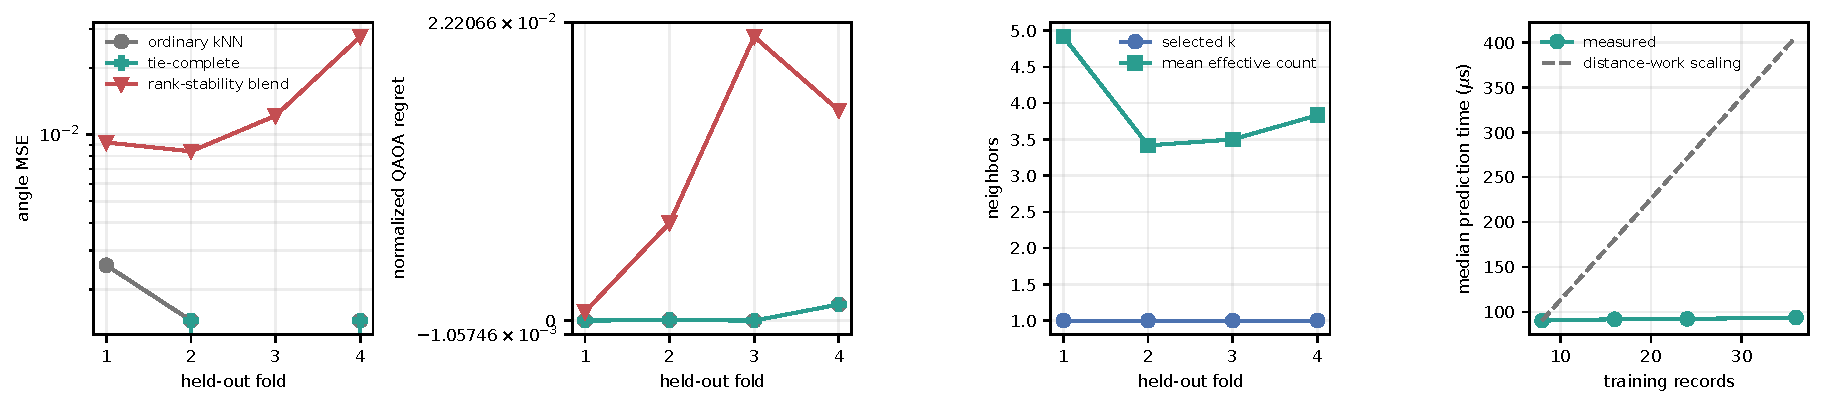
\includegraphics[width=\textwidth]{code/results/figures/tie_neighbor_audit.pdf}
\caption{\label{fig:ties}Row-held-out audit.  The first two panels separate
angle error from energy regret.  The third reports selected $k$ and the larger
effective neighbor count caused by complete distance ties.  The final panel
times twelve real queries against prefixes of the actual training partition;
fixed overhead dominates this small range despite the increasing distance
work.}
\end{figure}

\begin{figure}[t]
\centering
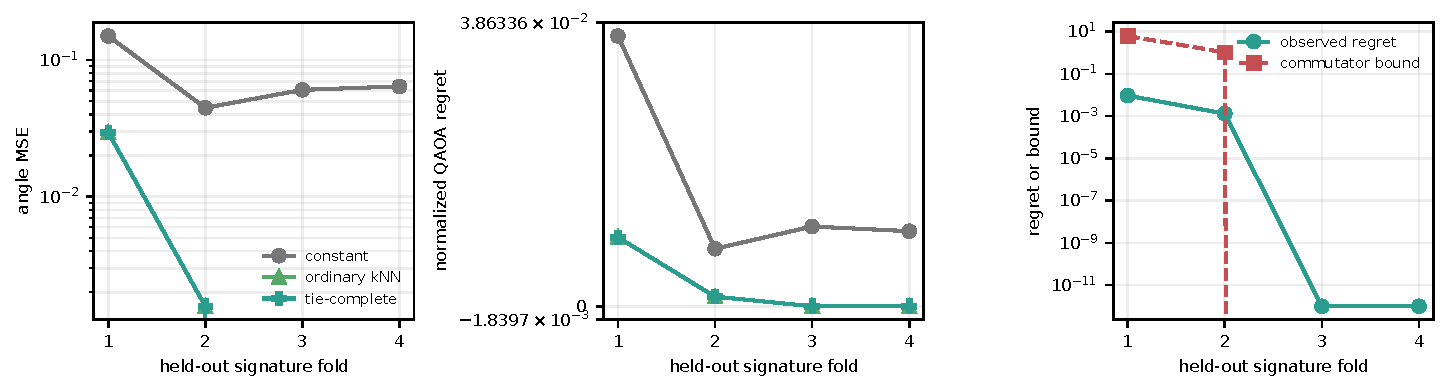
\includegraphics[width=0.94\textwidth]{code/results/figures/signature_generalization.pdf}
\caption{\label{fig:signature}Collision-free signature-grouped evaluation.
Left and center: foldwise angle error and energy regret.  Right: observed
tie-complete regret and the commutator certificate from
Theorem~\ref{thm:energy}.  The bound has no violations but is conservative.}
\end{figure}

\section{Interpretation and reproducibility}

The tie-complete rule solves a well-defined reproducibility defect: serialized
row order cannot decide among equal-distance graph signatures.  Its advantage
on the row split is real but arises from exact-signature reuse.  The
signature-held-out experiment supplies no evidence that tie completion itself
improves extrapolation; ordinary and tie-complete neighbors coincide there.
Nor does a coarse-grid parameter label establish a continuous optimizer.

The package records G1 and G81 source addresses and byte hashes, all
neighborhoods, grid settings, folds, signature groups, selected neighbor
counts, effective tie counts, per-fold errors, energy certificates, timing
samples, and locked outputs.  The authenticated replay reconstructs all
48 landscapes, regenerates the tables and figures, and compares every
non-timing value with the committed result.  Tests additionally permute tied
training rows and verify prediction invariance.

\bibliographystyle{plainnat}
\bibliography{code/manuscript_assets/references}

\end{document}
